\documentclass[12pt,letter]{article}


\usepackage{nicefrac,amsmath}
\usepackage[english]{babel}
\usepackage{helvet}
\usepackage{enumerate}
\usepackage{parskip}
%\usepackage{apacite}
\usepackage[english]{babel}
\usepackage{booktabs}
\usepackage[top=1in, bottom=1in, left=1in, right=1in]{geometry}
\usepackage{graphicx}
\usepackage{subfigure}
\usepackage{url}
\usepackage{hyperref}
\usepackage{physics}
\usepackage{cancel}
\usepackage{gensymb}
\usepackage{bbm}
\usepackage{dsfont}
\usepackage{mathtools}
\usepackage{appendix}
\usepackage{etoolbox}

\usepackage{amsfonts}

% Inserts \clearpage before \begin{appendices}
\BeforeBeginEnvironment{appendices}{\clearpage}

\usepackage{algpseudocode}
\usepackage{algorithm}


\usepackage[usenames,dvipsnames]{color}
 \usepackage{listings}
 \definecolor{Brown}{cmyk}{0,0.81,1,0.60}
 \definecolor{OliveGreen}{cmyk}{0.64,0,0.95,0.40}
 \definecolor{CadetBlue}{cmyk}{0.62,0.57,0.23,0}



 \lstset{language=C,%basicstyle=\normalsize,
 keywordstyle=\ttfamily\color{OliveGreen}\bfseries,
 identifierstyle=\ttfamily\color{CadetBlue}\bfseries, 
 commentstyle=\color{Brown}\ttfamily,
 stringstyle=\ttfamily\color{red},
 showstringspaces=false}


\newcommand{\argmax}[1]{\underset{#1}{\operatorname{arg}\,\operatorname{max}}\;}
\newcommand{\argmin}[1]{\underset{#1}{\operatorname{arg}\,\operatorname{min}}\;}



%\usepackage{cmbright}
\usepackage[T1]{fontenc}

\usepackage{xcolor}
\usepackage{mdframed}



\setlength{\parskip}{12pt} % 1ex plus 0.5ex minus 0.2ex}

%\renewcommand{\familydefault}{\sfdefault}

\setlength{\parindent}{0cm}
\renewcommand{\baselinestretch}{1.2}

\title{{\bf Calculus Review: Functions} }
%\author{CSE5280}

\date{}
\begin{document}
\maketitle
\vspace{-1.0in}

%{\small 
%\tableofcontents
%%\listoffigures
%%\listofalgorithms
%}

%\newpage

\section{Overview}
In mathematics, a function describes the relationship between a quantity that is dependent on another quantity (e.g., position as a function of time, yearly income as a function of worked hours). These quantities are called {\em variables}, which can be either {\em dependent} or {\em independent}. 

The dependent variable, which is the value of the function itself, describes the value of the quantity that depends on the other variables. Independent variables do not depend on other variables. Functions can only have one value of the dependent variable for each value of the independent variable. Mathematically, we denote a function as $f$ and its value as $f(x)$. Here, $f$ is the dependent variable and $x$ is the independent variable. Note that it is common for some people to ``abuse the notation" a bit and refer to $f(x)$ as a function when this is actually the value of the function at $x$. \\

    \begin{mdframed}[backgroundcolor=yellow!20] 
{\bf Definition}: A function is a mathematical relationship in which the values of a single dependent variable are determined by the values of one or more independent variables. Function means the dependent variable is determined by the independent variable(s).\footnote{http://www.columbia.edu/itc/sipa/math/variables.html}.
    \end{mdframed}



\section{Characterizing functions in terms of dimensionality}
In terms of the dimensionality of the variables, functions can be of the following types:

\begin{enumerate}
    \item A scalar function of a single scalar variable.
    \item A scalar function of multiple scalar variables (or a scalar function of a vector variable).
    \item A vector function of a single scalar variable.
    \item A vector function of a vector variable.
\end{enumerate}




\subsection{A scalar function of a single scalar variable}

In scalar functions of a single scalar variable, both the function value, $f(x)$, and its independent variable $x$ are real numbers, i.e.,  $f(x) \in \mathbb{R}$ and $x \in \mathbb{R}$. Figure \ref{fig_functionType1} shows an example. 	
\begin{figure}[H]
	\begin{center}
		{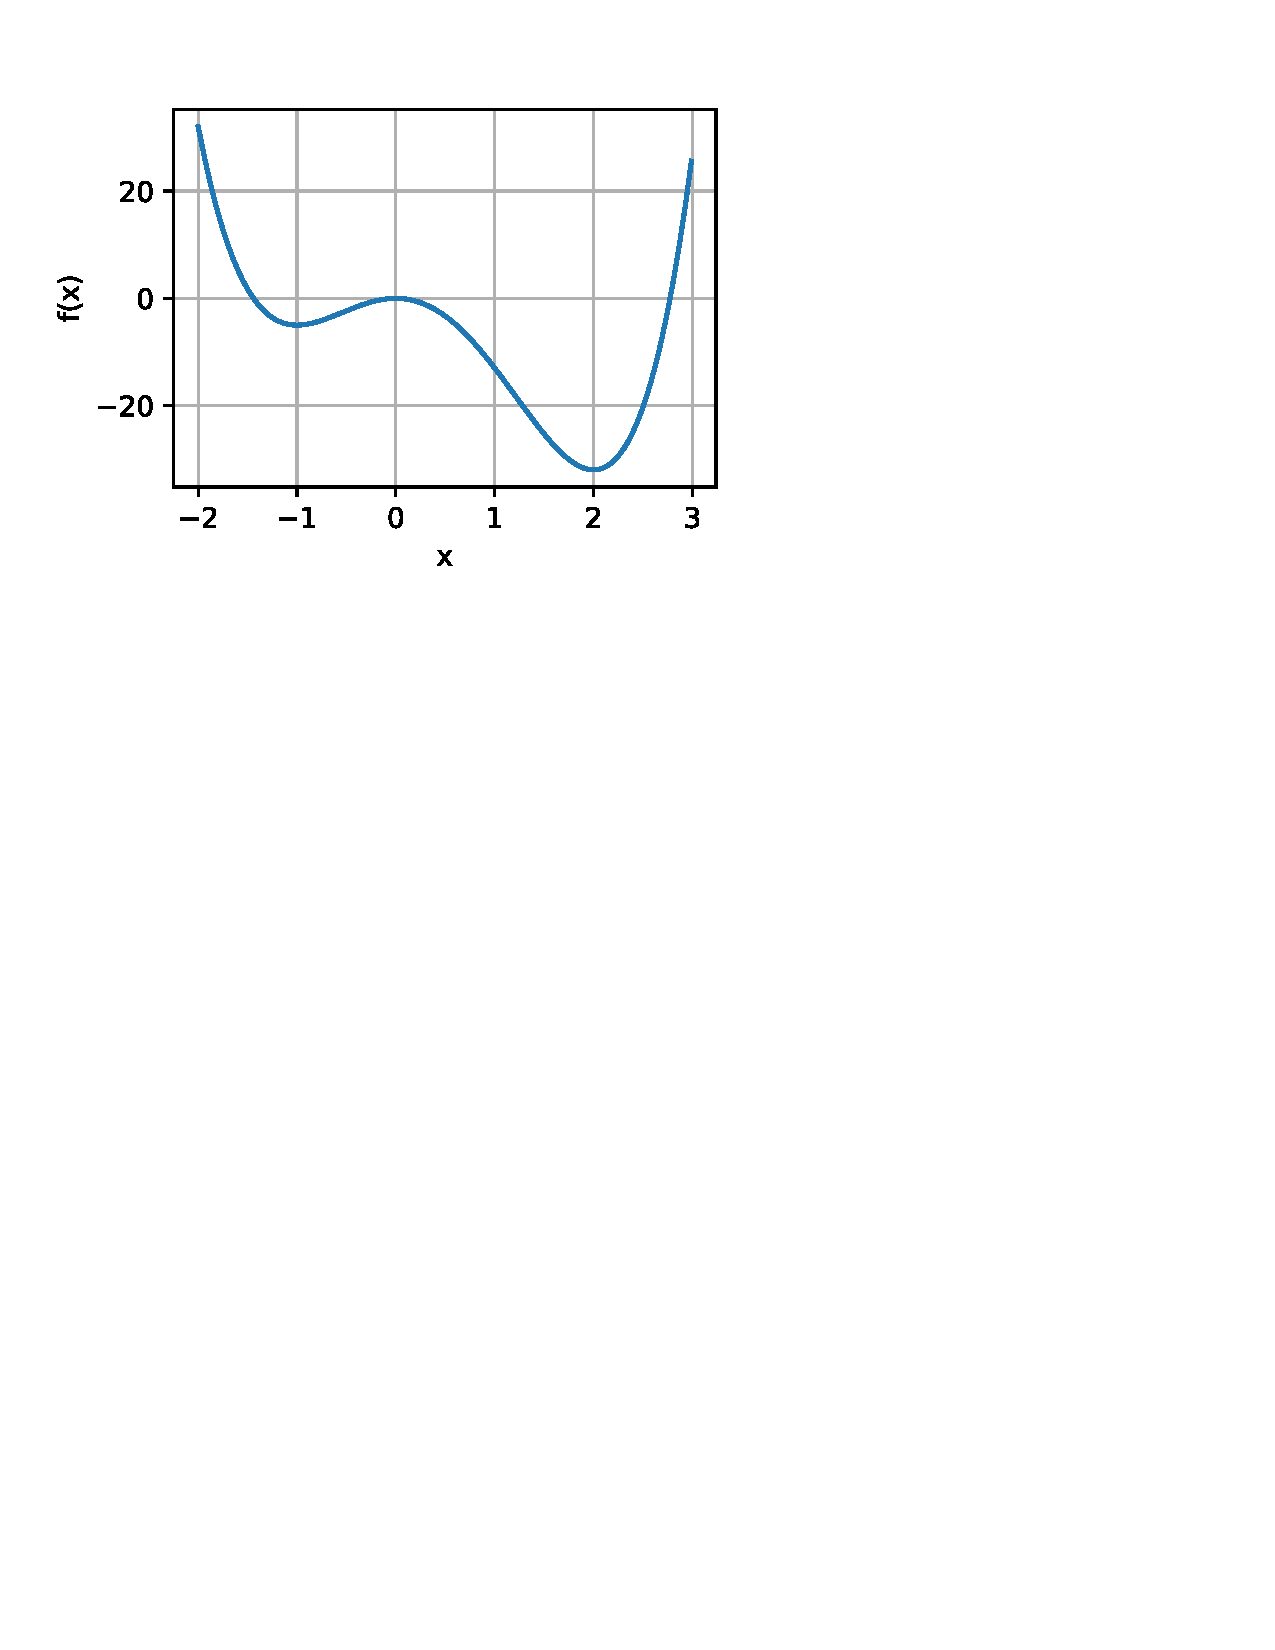
\includegraphics[width=.50\textwidth]{figs/scalarFunctionScalarVariable}}
	\end{center}
	\caption{A scalar function of a single scalar variable, $f(x) = 3x^4 - 4x^3 - 12x^2$.}
	\label{fig_functionType1}
\end{figure}
	%

\subsection{A scalar function of multiple scalar variables (or a scalar function of a vector variable)}

In this case, the function value $f({\bf x})$ is a (single) real number, which is dependent on multiple  independent variables ${\bf x} = \left(x_1,\hdots,x_n\right)^\mathsf{T}$, i.e.,  $f({\bf x}) \in \mathbb{R}$ and ${\bf x} \in \mathbb{R}^n$. A bold lowercase letter denotes a vector variable.
\begin{figure}[H]
	\begin{center}
		{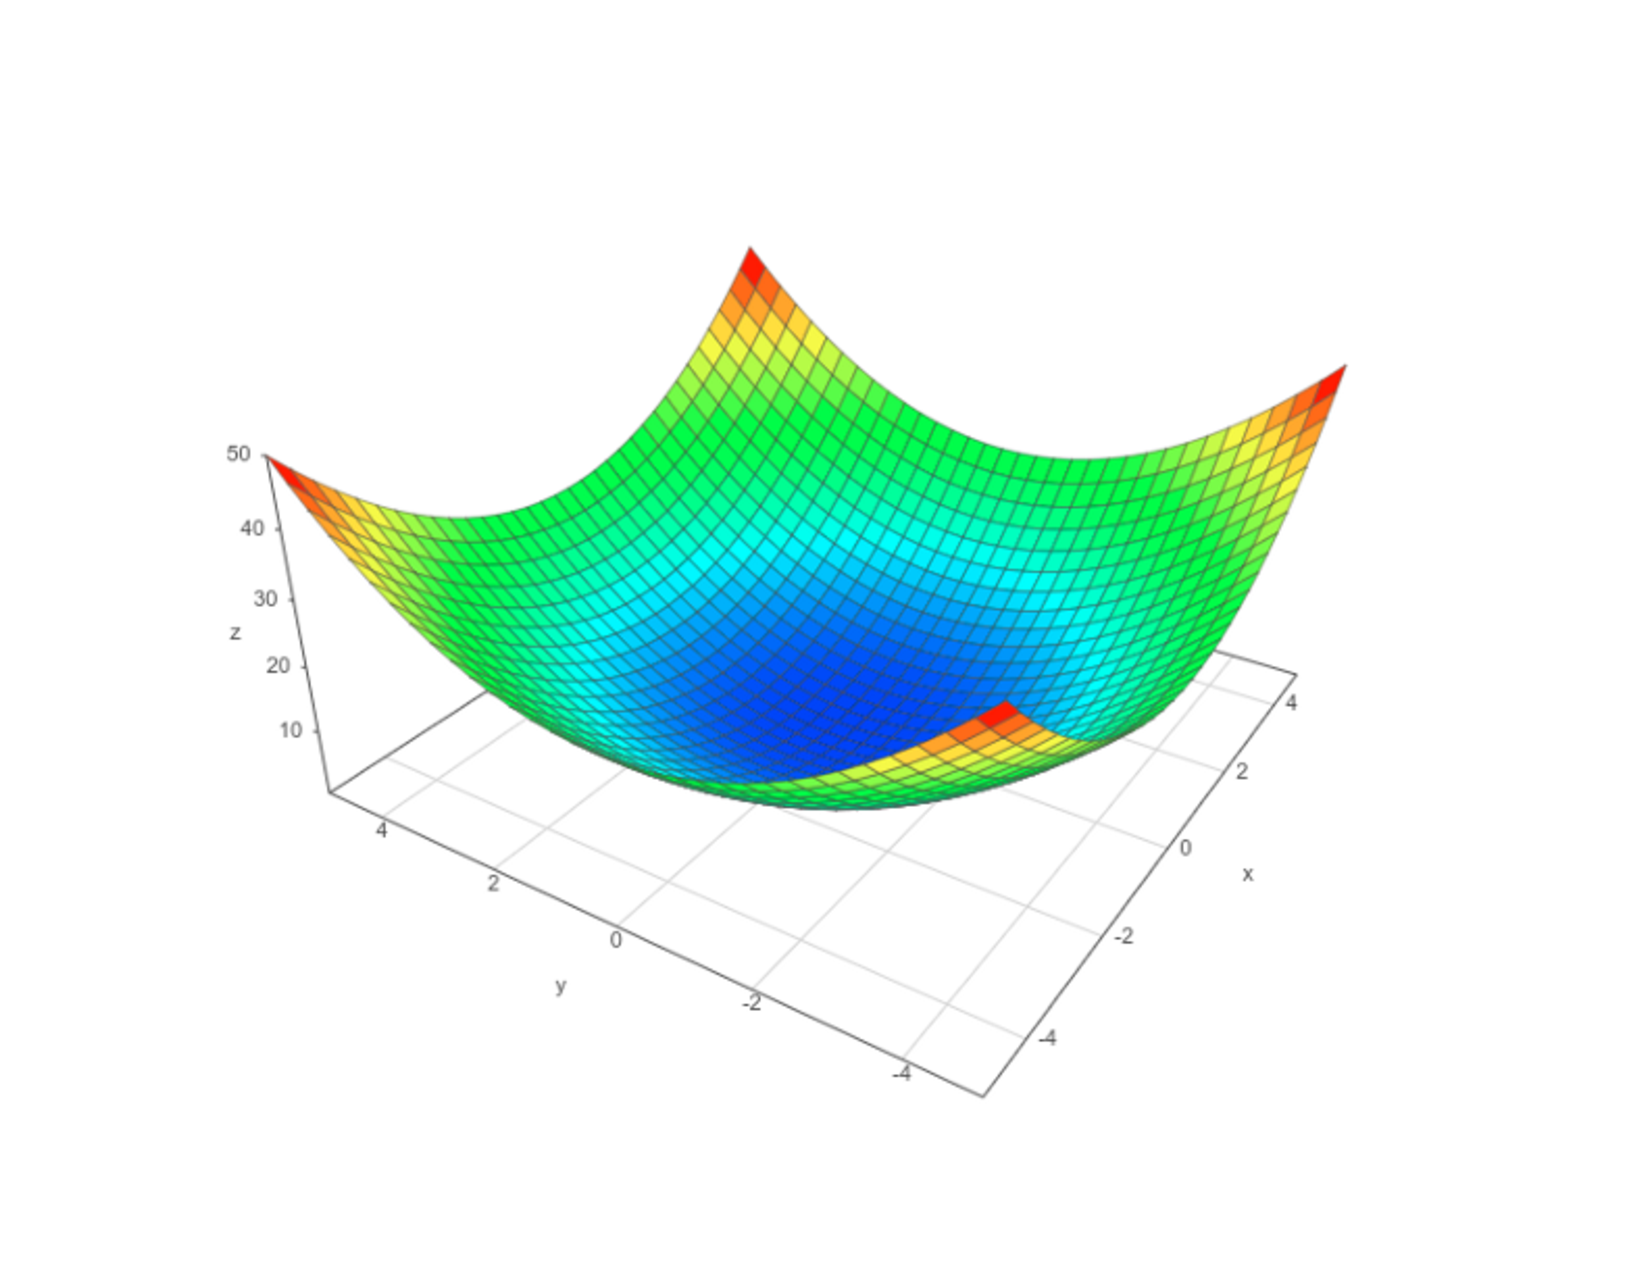
\includegraphics[width=.50\textwidth]{figs/scalarFunctionMultivariate}}
	\end{center}
	\caption{A scalar function of multiple variables (or vector variable), $f(x,y) = x^2 + y^2$.}
	\label{fig_functionType2}
\end{figure}
	% 
	
	
\newpage
\subsection{A vector function of a single scalar variable}

In these types of functions, it is the function value ${\bf f}(x)$ that is a vector ${\bf f}(x) = \left(x_1,\hdots,x_n\right)^\mathsf{T}$ (or multivariate). But, this value ${\bf f}(x)$ depends on a single scalar variable, i.e., ${\bf f}(x) \in \mathbb{R}^n$ and ${x} \in \mathbb{R}$. For example, the motion of a particle as a function of time.
\begin{figure}[H]
	\begin{center}
		{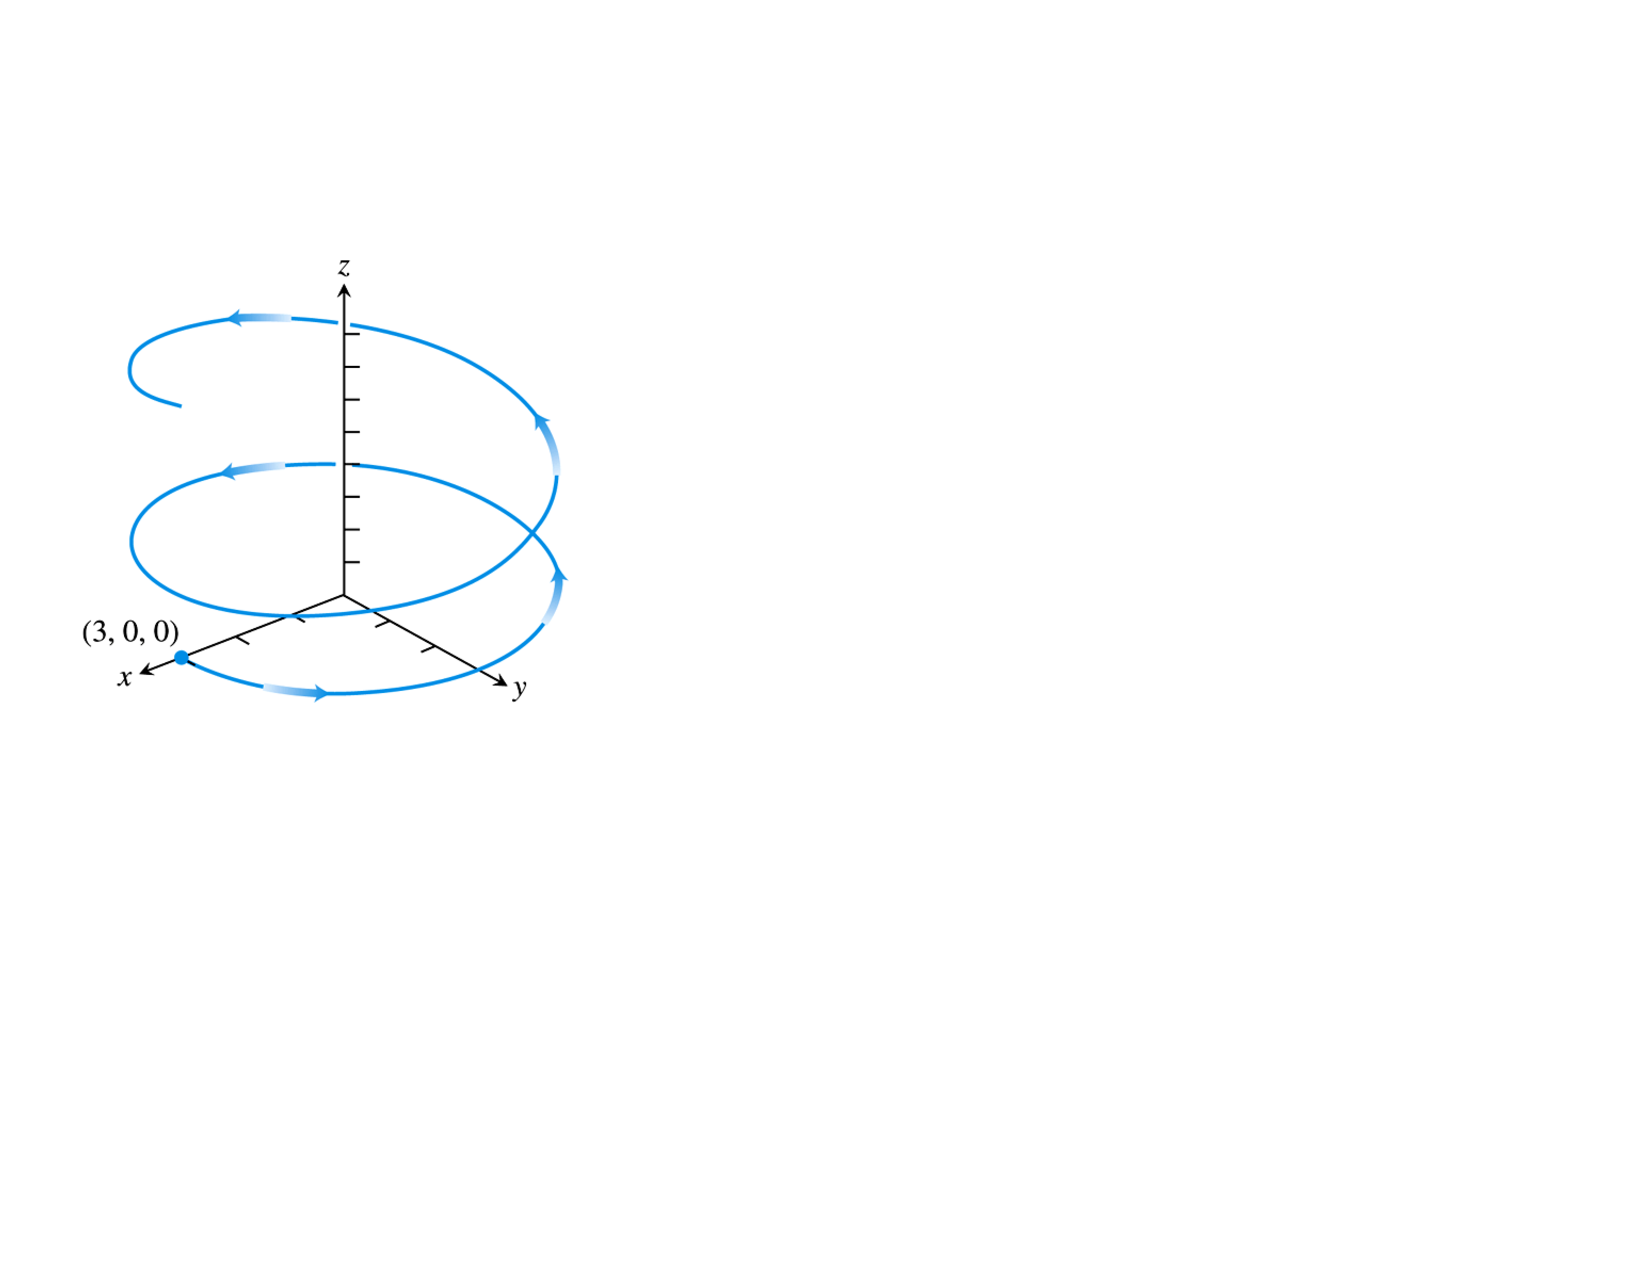
\includegraphics[width=.30\textwidth]{figs/hang_glider}}
	\end{center}
	\caption{A vector function of a scalar variable. The path of a hang glider with position vector 
	 ${\bf r}(t) = (3\cos t)\,{\bf i} + (3\sin t)\,{\bf j} + t^2\,{\bf k}$.}
	\label{fig_functionType3}
\end{figure}



	%
\subsection{A vector function of a vector variable} 

For some functions, both the dependent and independent variables are vectors (i.e., multiple dependent variables are dependent of multiple independent variables).  In this case, ${\bf f}$ is a vector-valued function of a vector of variables, ${\bf x}$. Here, ${\bf f}\left({\bf x}\right) = \left(f_1, f_2, \hdots, f_M\right)^\mathsf{T}$ and ${\bf x} = \left(x_1, x_2, \hdots, x_N\right)^\mathsf{T}$, with ${\bf f}({\bf x}) \in \mathbb{R}^n$ and ${\bf x} \in \mathbb{R}^n$. Figure \ref{fig_functionType4} shows an example of the motion of an articulated robot arm. The arm's pose  and the 3-D location of its tip are given in terms of a set of joint angles. The figure also shows that a vector function of a vector variable describes a vector field. 
\begin{figure}[H]
	\begin{center}
		{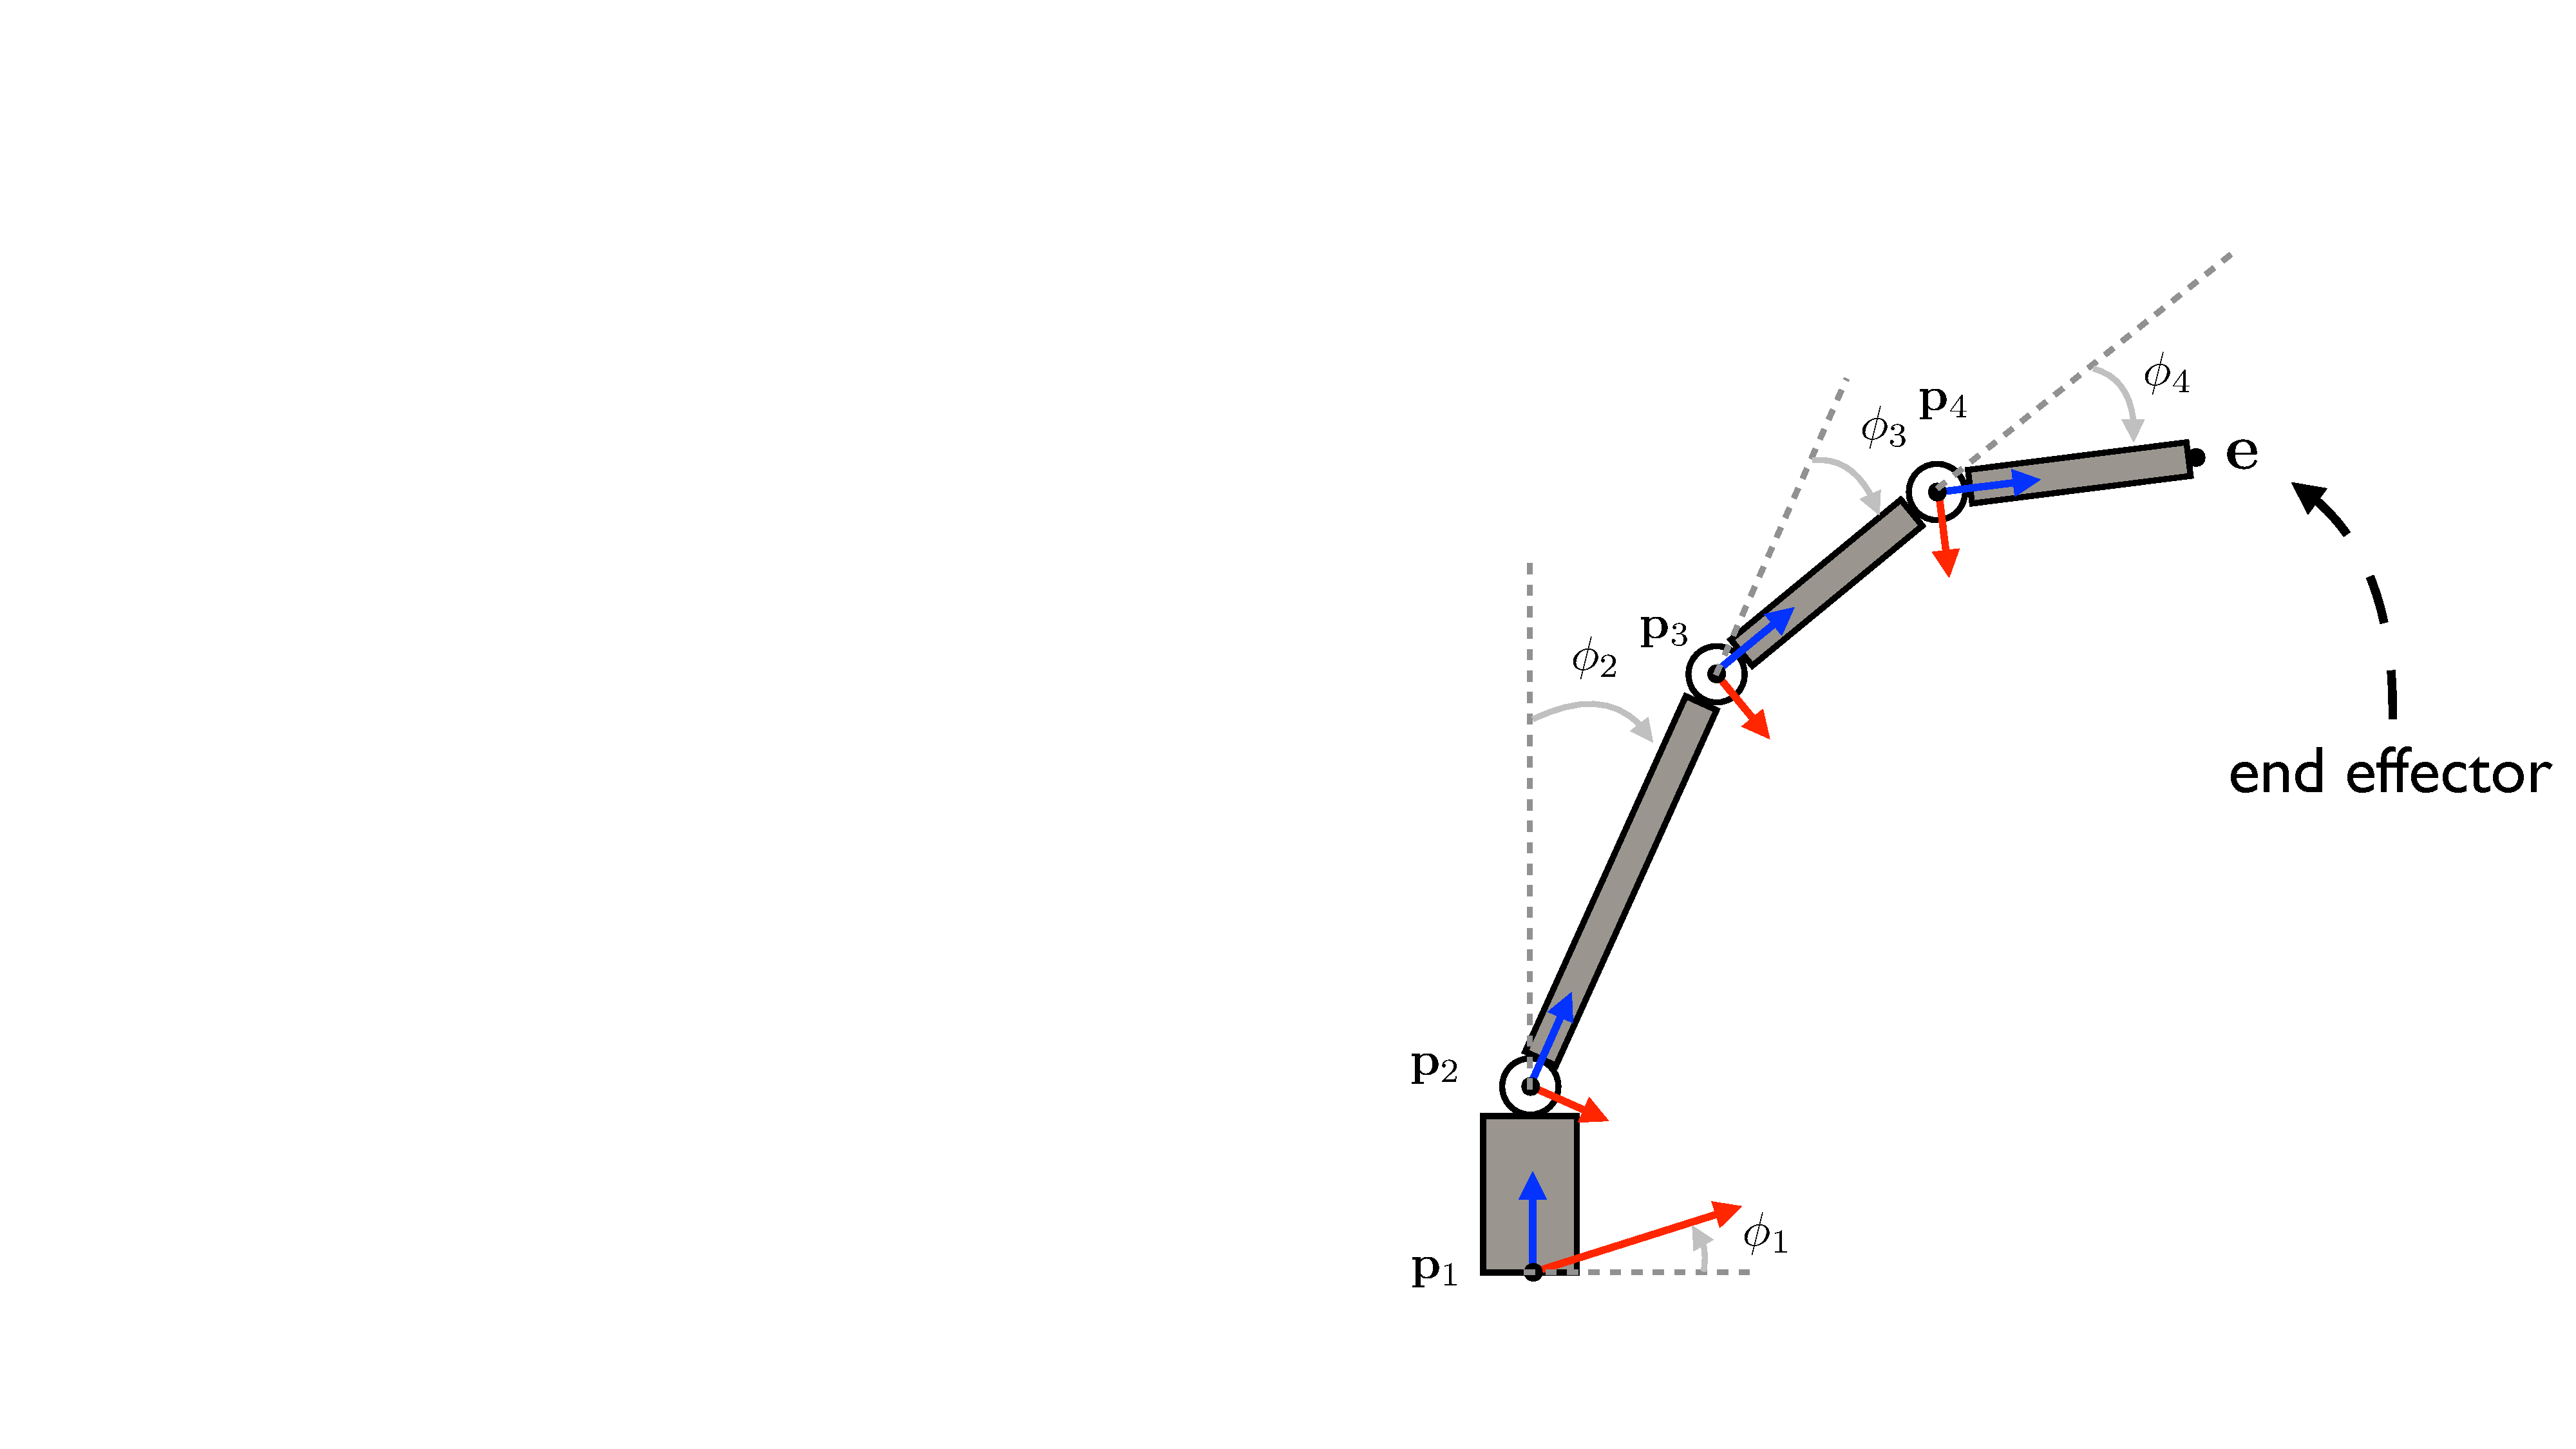
\includegraphics[width=.32\textwidth]{figs/robotArm}}
		{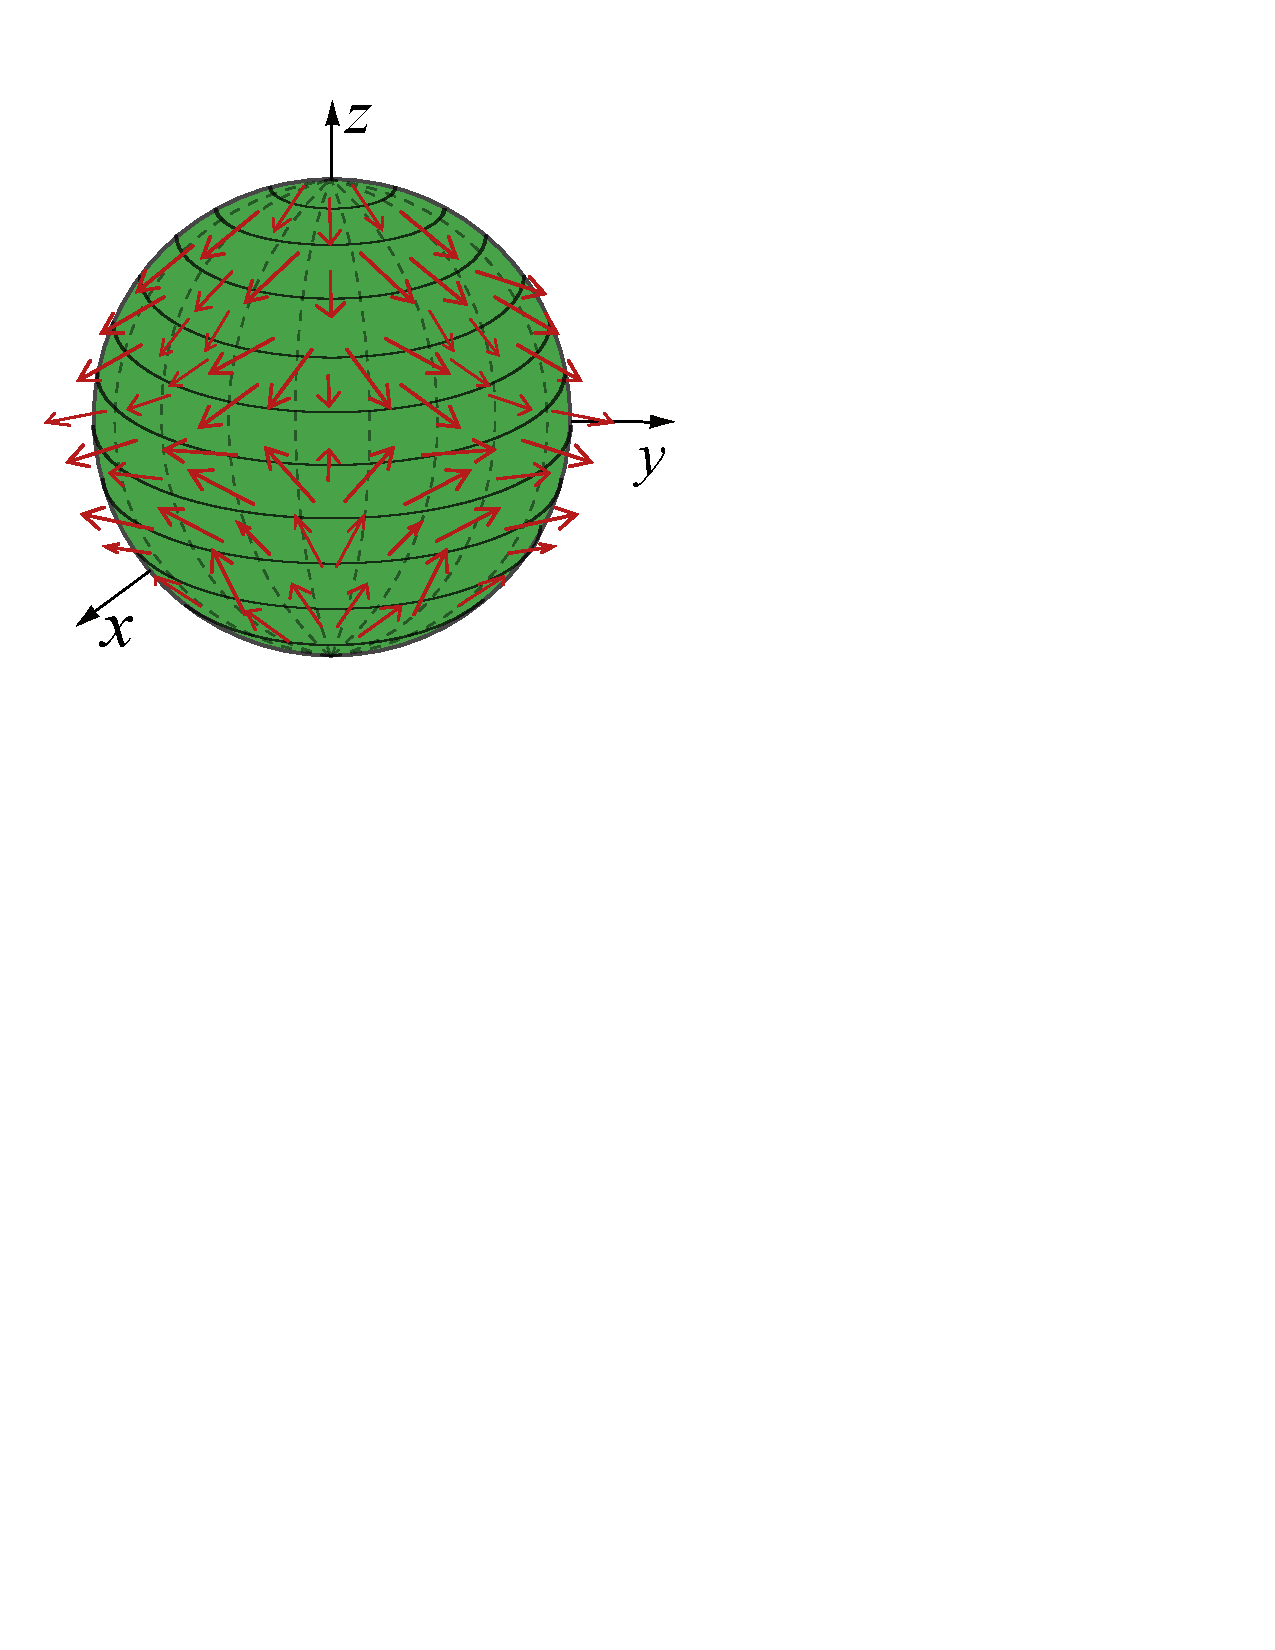
\includegraphics[width=.32\textwidth]{figs/vectorFieldSphere}}				
	\end{center}
	\caption{Vector functions of a vector variable. A robot arm and a vector field on a sphere (Figure from: \url{https://en.wikipedia.org/wiki/Vector_field}).}
	\label{fig_functionType4}
\end{figure}
	
	



%\section{Derivative of a scalar function of a single scalar variable}
%
%Let $f$ be a scalar function of a single variable $x$. The derivative of the function w.r.t. $x$ is: 
%\begin{align}
%        \dv{f}{x} = \lim_{\Delta x \rightarrow 0}\frac{\Delta f}{\Delta x} = \lim_{\Delta x \rightarrow 0}\frac{f\left(x+\Delta x\right) - f\left(x\right)}{\Delta x}.
%	\label{dfx}
%\end{align}	
%The derivative of a scalar function describes the slope (i.e., rate of change) of the function at a given point $x$. Figure \ref{fig_dfdx} shows the derivative of the function $f(x) = x\sin x^2 + 1$ at $x=-1$, $-0.5$, $1$, $0.5$, and $1$. The derivative of the function is $\dfrac{df}{dx}\left(x\right) = 2x^2\cos x^2 + \sin x^2$.
%\begin{figure}[ht]
%	\begin{center}
%		{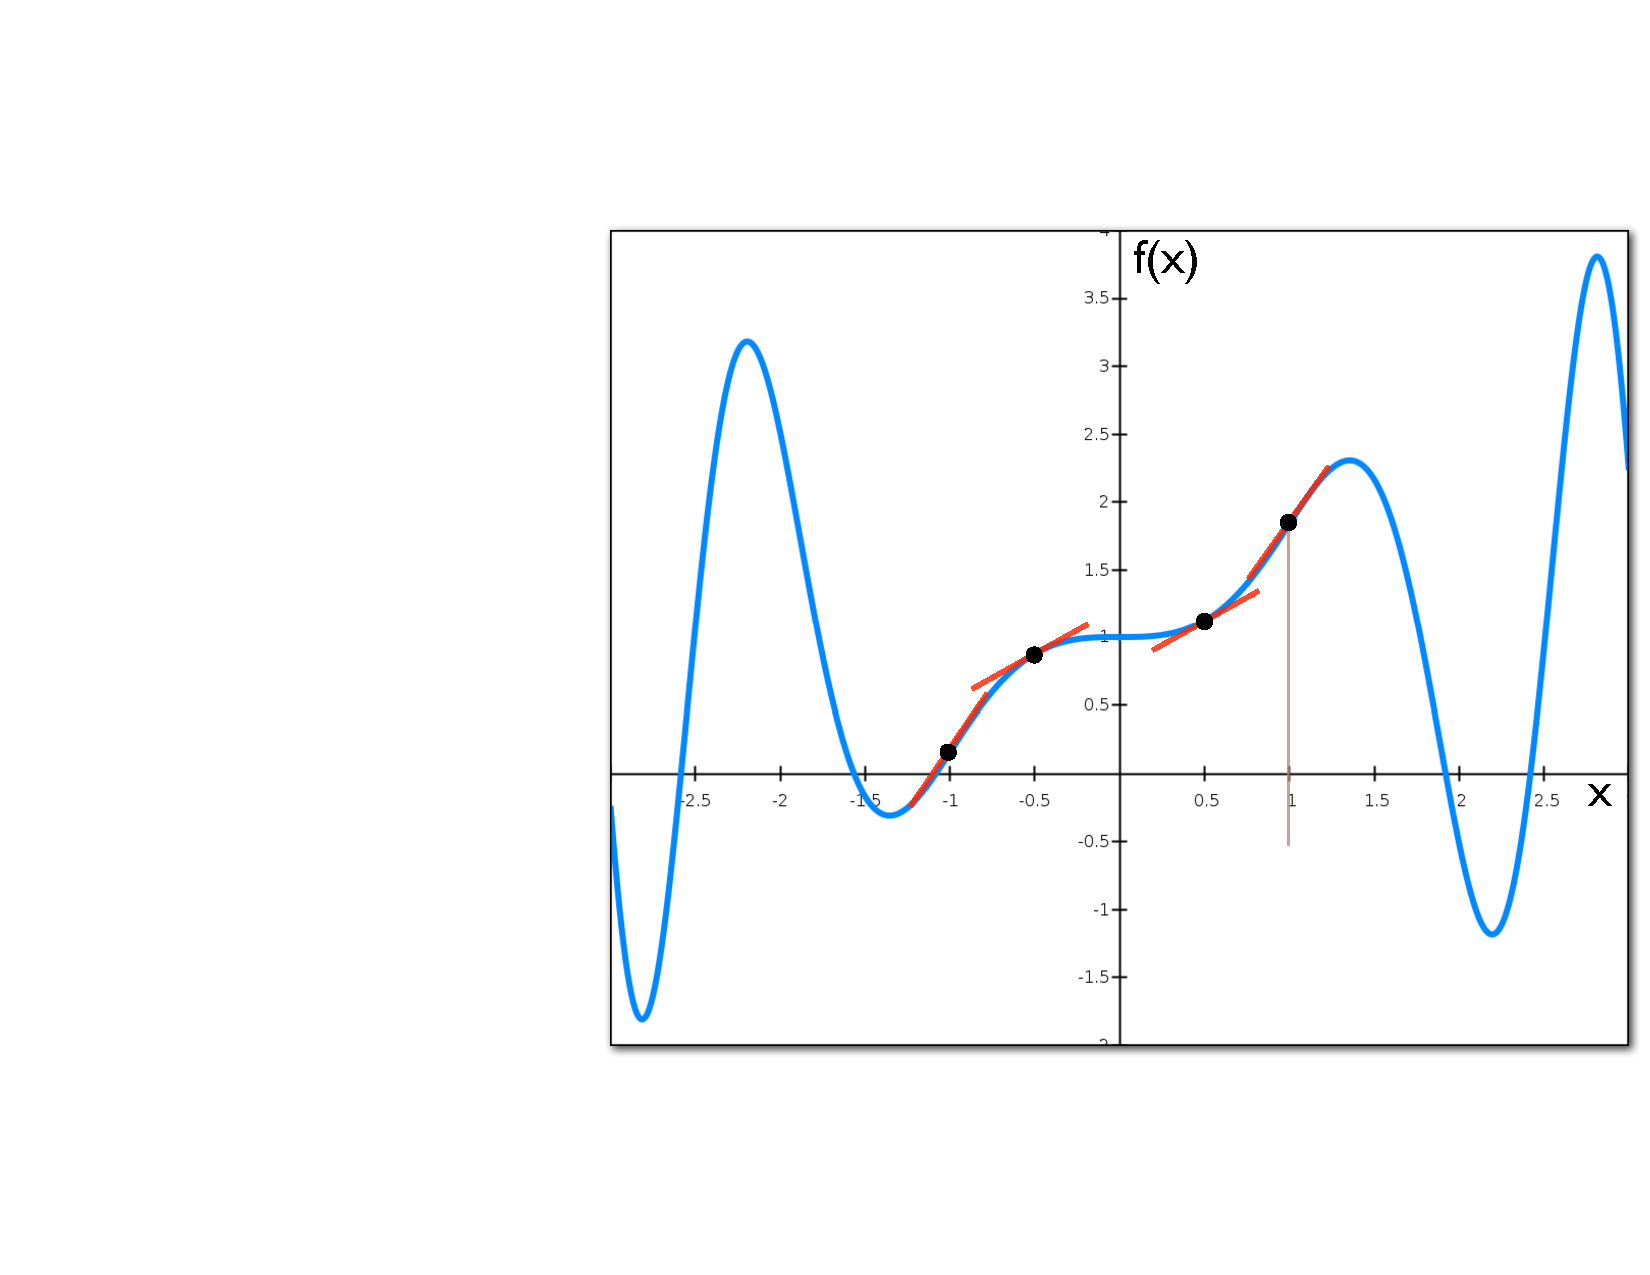
\includegraphics[width=.80\textwidth]{figs/derivative.pdf}}
%	\end{center}
%	\caption{The derivative of the function $f(x) = x\sin x^2 + 1$ at $x=-1$, $-0.5$, $1$, $0.5$, and $1$. }
%	\label{fig_dfdx}
%\end{figure}
%
%%\section{Derivative approximation}
%%
%%Often, calculating the derivative  analytically can be very hard. In these cases, we can make progress by approximating the derivative numerically by using discrete differences. In fact, as long as we can evaluate the function, we can always approximate the derivative, i.e.: 
%%\begin{align}
%%        \dv{f}{x} \approx \frac{\Delta f}{\Delta x} = \frac{f\left(x+\Delta x\right) - f\left(x\right)}{\Delta x},
%%	\label{approx}
%%\end{align}	
%%for a small $\Delta x$. Figure \ref{fig_dfdx_approx} shows the approximate derivative of the function for a small $\Delta x$. 
%%
%%\begin{figure}[ht]
%%	\begin{center}
%%		{\includegraphics[width=.80\textwidth]{figs/derivative_approx.pdf}}
%%	\end{center}
%%	\caption{The approximate derivative of the function $f(x) = x\sin x^2 + 1$ at $x=-1$. }
%%	\label{fig_dfdx_approx}
%%\end{figure}
%%
%%
%%\section{Calculating the value of functions at nearby points}
%%
%%Another useful tool from derivatives is that it allows us to calculate the value of a function at nearby points. Given the value of a function at a point, $f(x)$, and its derivative, $df/dx$, we can estimate the value of the function at a point near $x$, i.e.: 
%%\begin{align}
%%        \frac{\Delta f}{\Delta x} &\approx \dv{f}{x}   \notag  \\ 
%%         {\Delta f} &\approx  {\Delta x} \dv{f}{x}  \notag \\ 
%%         f\left(x+\Delta x\right) - f\left(x\right) &\approx  {\Delta x} \dv{f}{x}  \notag \\ 
%%         f\left(x+\Delta x\right) &\approx   f\left(x\right) + {\Delta x} \dv{f}{x}.  
%%	\label{nearby}
%%\end{align}	
%%
%%\begin{figure}[ht]
%%	\begin{center}
%%		{\includegraphics[width=.80\textwidth]{figs/derivative_nearby_point}}
%%	\end{center}
%%	\caption{Derivatives allow us to calculate the value of a function at nearby points. Given the value of a function at a point, $f(x)$, and its derivative, $df/dx$, we can estimate the value of the function at a point near $x$ }
%%	\label{fig_nearby_point}
%%\end{figure}
%%
%%
%%\section{The gradient-descent method}
%%\label{grad_descent_scalar_function}
%%
%%Many times, we want to find the value for which a function is zero, i.e., we want to find solutions to the equation $f\left(x\right) = 0$. This equation can be solved analytically or numerically. One of the many numerical methods to solving this equation is the gradient-descent method. 
%%
%%\begin{figure}[ht]
%%	\begin{center}
%%		{\includegraphics[width=.80\textwidth]{figs/nearby_point_g}}
%%	\end{center}
%%	\caption{Computing the gradient descent's $\Delta x$ step. The red arrow shows a step that was computed  using ${\Delta x} = \left(g - f\left(x_i\right) \right) \left(\dv{f}{x}\right)^{-1}$, which may be too large (and over optimistic) given the function's linear approximation $df/dx$. In contrast, the green arrow shows a (smaller) step that was computed using ${\Delta x} = \beta\left(g - f\left(x_i\right) \right) \left(\dv{f}{x}\right)^{-1}$, with $0<\beta\leq 1$. For instance, we can set $\beta = 0.1$.}
%%	\label{fig_nearby_point_g}
%%\end{figure}
%%
%%
%%If we can evaluate $f\left(x\right)$ and $df/dx$ for any value of $x$, we can always follow the slope (i.e., gradient) in the direction towards 0. Starting at some initial value $x_0$, take small steps until we find a value $x_n$ for which $f\left(x_n\right) = 0$. 
%%\begin{align}
%%        x_{i+1} = x_i + \Delta x. 
%%	\label{steps}
%%\end{align}	
%%For each step, we choose a value of $\Delta x$ that brings us closer to our goal. We can try to choose $\Delta x$ to bring us closer to where the slope passes through 0, i.e.: 
%%\begin{align}
%%        \frac{\Delta f}{\Delta x} &\approx \dv{f}{x}   \notag  \\ 
%%         {\Delta f} &\approx  {\Delta x} \dv{f}{x}  \notag \\ 
%%         {\cancelto{0}{f\left(x_i+\Delta x\right)}} - f\left(x_i\right) &\approx  {\Delta x} \dv{f}{x}  \notag \\ 
%%          - f\left(x_i\right) &\approx  {\Delta x} \dv{f}{x}  \notag \\   
%%          {\Delta x}  &= - f\left(x_i\right) \left(\dv{f}{x}\right)^{-1}.     
%%	\label{choosingDeltax}
%%\end{align}	
%%
%%If we want to find where a function equals some value $g$ instead of $0$, we can think of the problem as minimizing $f\left(x\right) - g$ and just step towards $g$, i.e.: 
%%\begin{align}
%%          {\Delta x}  &= \left(g - f\left(x_i\right) \right) \left(\dv{f}{x}\right)^{-1}.
%%	\label{choosingDeltaxStepToG}
%%\end{align}	
%%
%%
%%
%%However, Equation \ref{choosingDeltaxStepToG} assumes that our linear approximation of the function given by its derivative is reliable for large values of $\Delta x$. However, this is not the case for non-smooth functions with varying derivatives. A safer way to choosing $\Delta x$ is to multiply it by a parameter $\beta \in \left(0,1\right]$ to scale the step. With the inclusion of the $\beta$ scale factor, Equation \ref{choosingDeltaxStepToG} can be re-written as:  
%%\begin{align}
%%          {\Delta x}  &= \beta \left(g - f\left(x_i\right) \right) \left(\dv{f}{x}\right)^{-1}.
%%	\label{scaledDeltaxStepToG}
%%\end{align}	
%% Figure \ref{fig_nearby_point_g} shows the $\Delta x$ steps computed  by using Equations \ref{choosingDeltaxStepToG} and \ref{scaledDeltaxStepToG}.
%%
%%
%%
%%
%%\begin{algorithm}[ht] % enter the algorithm environment
%%\caption{Gradient descent (scalar function of a single scalar variable)} % give the algorithm a caption
%%\label{algo_grad_descent} % and a label for \ref{} commands later in the document
%%\begin{algorithmic}[1]
%%	\State {$x_0 \gets \text{starting value}$} 
%%	\State {$f_0 \gets f\left(x_0\right)$} 
%%	\Comment {Evaluate $f$ at $x_0$}
%%\While  {$f_n \neq g$}     
%%	\State {$s_i \gets \dv{f}{x}\left(x_i\right)$} \Comment{Compute slope}
%%	\State {$x_{i+1} \gets x_i +\beta \left(g - f_i \right) \frac{1}{s_i}$} \Comment{Take a step along $\Delta x$}
%%	\State {$f_{i+1} \gets f\left(x_{i+1}\right)$} \Comment{Evaluate $f$ at new $x_{i+1}$}
%%\EndWhile
%%\end{algorithmic}
%%\end{algorithm}
%%
%\section{Derivative of a scalar function of multiple scalar variables (i.e., vector variable)}
%
%Let $f$ be a scalar function of a vector variable. The vector variable is ${\bf x} = \left(x_1, x_2, \dots, x_N\right)^\mathsf{T}$. This type of function is also called a scalar function of multiple variables or multi-variate function. The value of the function at a point ${\bf x}$ is given by $f\left({\bf x}\right)$ or  $f\left(x_1, x_2, \dots, x_N\right)$, and its derivative w.r.t. $x$ is: 
%\begin{align}
%        \dv{f}{\bf x} =  \grad f = \pdv{f}{\left(x_1, x_2, \dots, x_N\right)} = \left[ \pdv{f}{x_1}\,\,  \pdv{f}{x_2}\,\, \cdots \,\,\pdv{f}{x_N}\right]^\mathsf{T}, 
%	\label{gradient}
%\end{align}	
%which is called the {\em Gradient} of $f$ at $x$, and denoted by $\grad f$. An example of a gradient vector field of a function $f(x_1,x_2)$ is shown in Figure \ref{fig_grad}. 
%
%\begin{figure}[ht]
%	\begin{center}
%		\subfigure[]{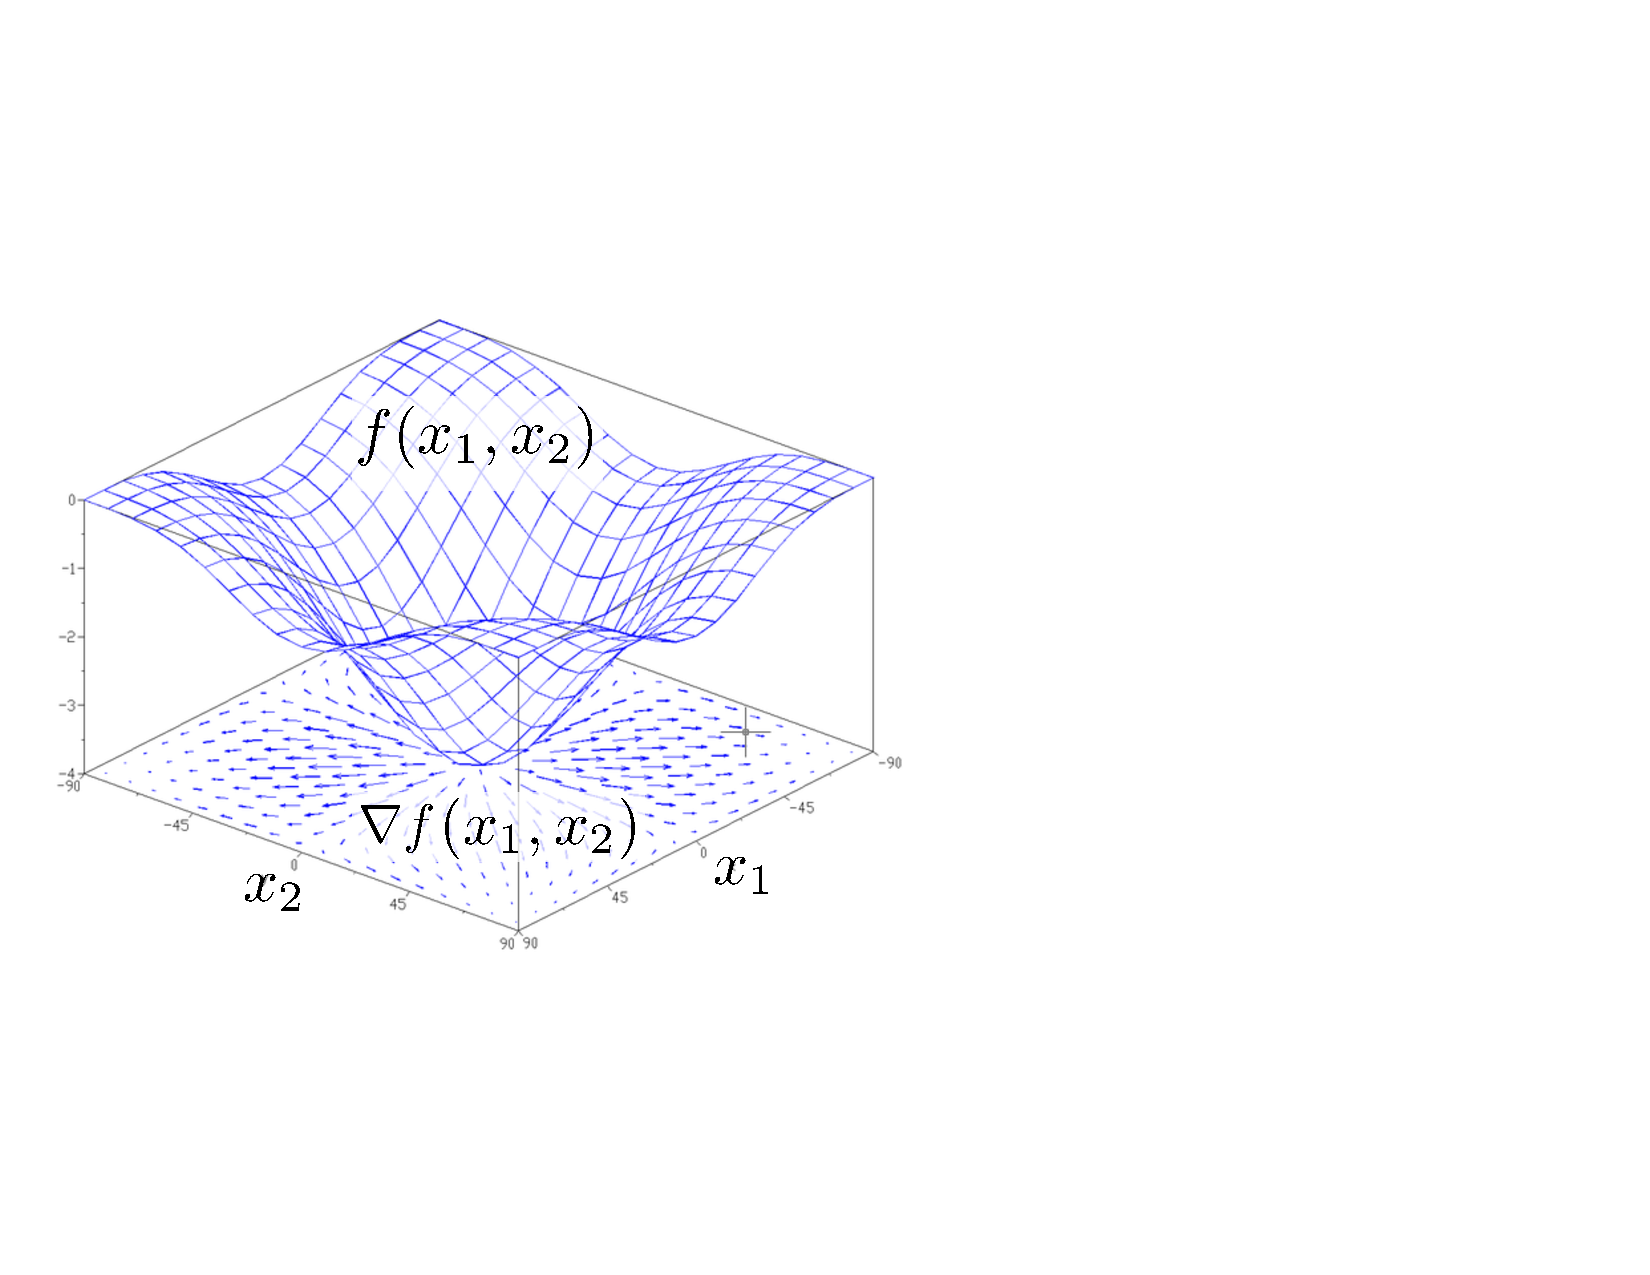
\includegraphics[width=.48\textwidth]{figs/grad_fig}}
%		\subfigure[]{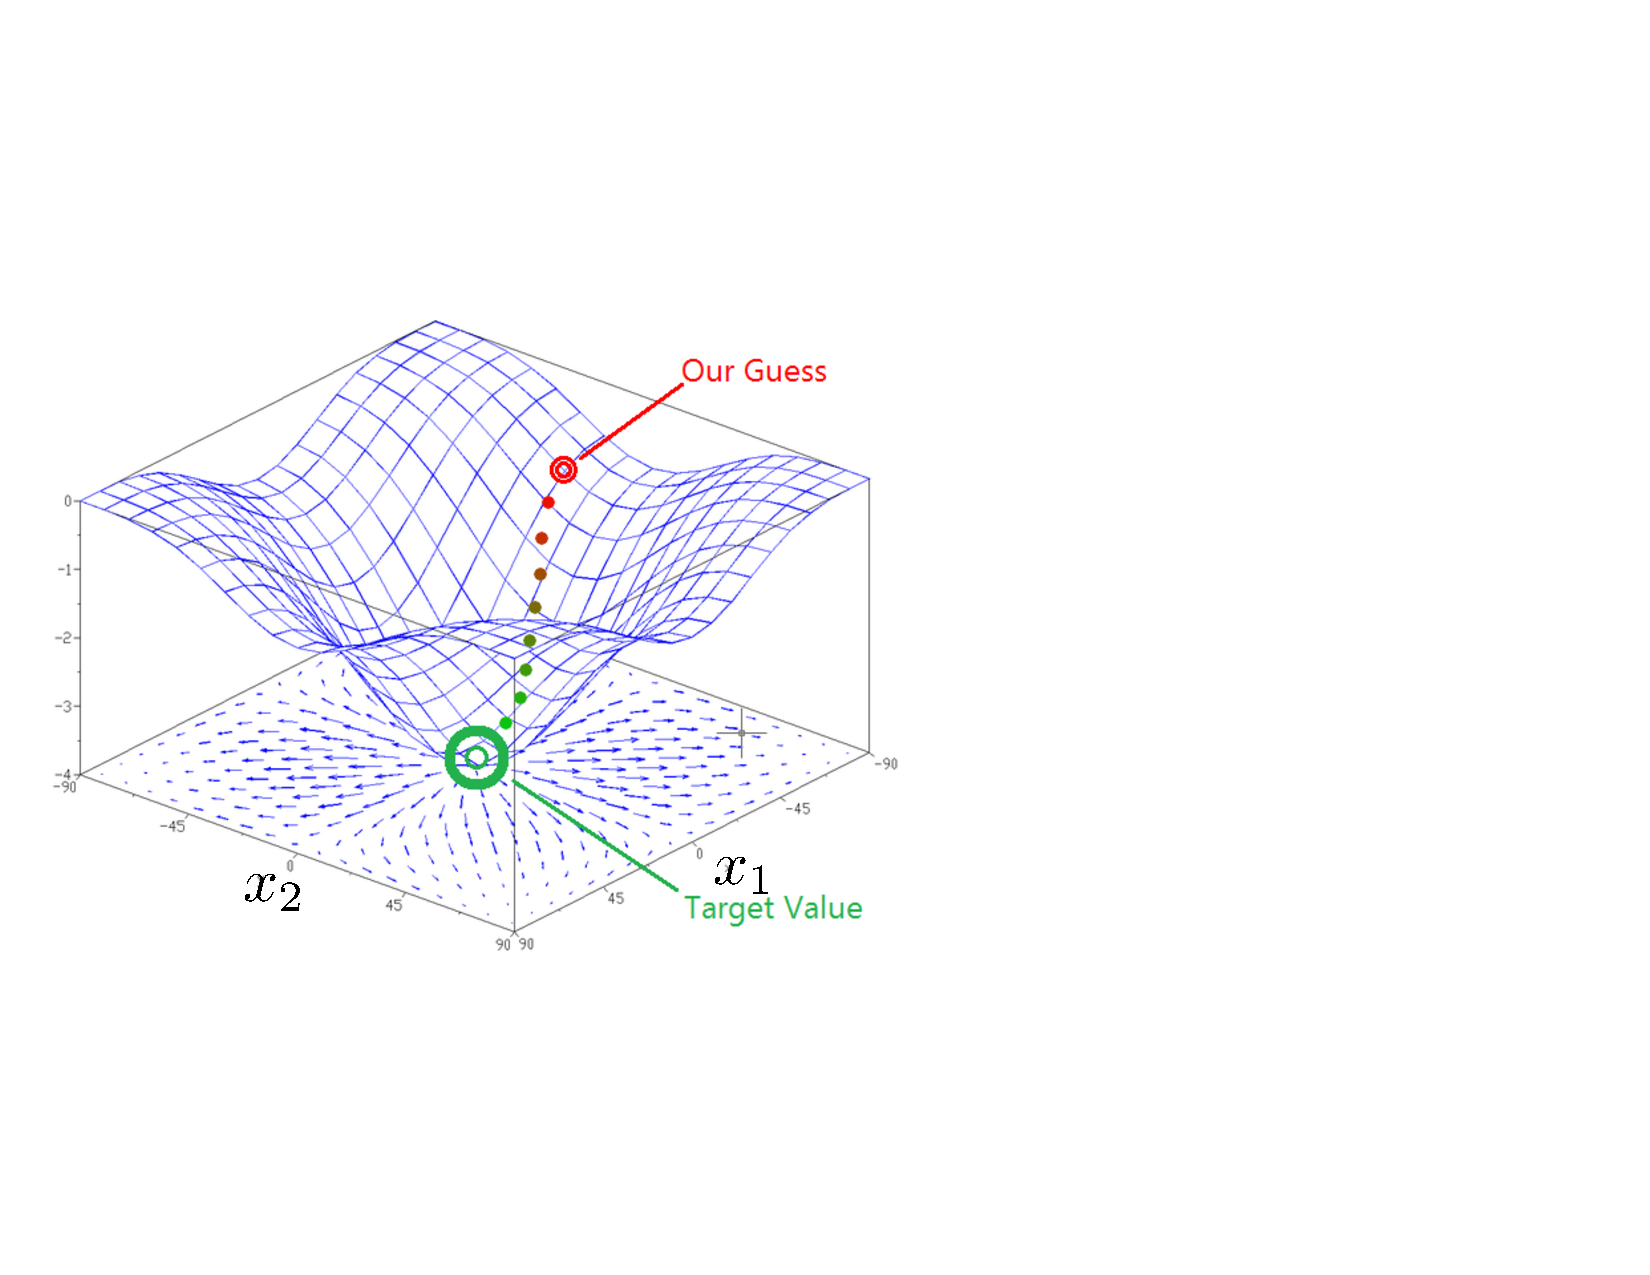
\includegraphics[width=.48\textwidth]{figs/grad_descent_fig}}
%	\end{center}
%	\caption{(a) Gradient vector field of two-variate function. (b) Gradient-descent method. In the gradient-descent method, we want to take the direction inverse to the gradient as the gradient (slope) points ``uphill''. Plots adapted from \url{https://goo.gl/zejgBw}.}
%	\label{fig_grad}
%\end{figure}
%
%
%\section{Derivative of a vector function of a single scalar variable}
%
%Let ${\bf r}$ be a vector function representing the 3-D motion of a particle as a function of time $t$: 
%\begin{align}
%          {\bf r}  &= \left[ r_x\,\,  r_y\,\,  r_z \right]^\mathsf{T}.
%	\label{particle_motion}
%\end{align}
%Its derivative is given by: 
%\begin{align}
%          \dv{\bf r}{t}  &= \left[ \dv{r_x}{t}\,\,  \dv{r_y}{t}\,\,  \dv{r_z}{t} \right]^\mathsf{T}, 
%	\label{derivative_particle_motion}
%\end{align}
%which is also a vector representing the velocity of the particle at time $t$. 
%
%
%
%
%
%\section{Derivative of a vector function of a vector variable}
%\label{sec_jacobian}
%
%Some applications require us to calculate derivatives of vector quantifies with respect to other vector quantities. For example, if ${\bf f}$ is a vector-valued function of a vector of variables, ${\bf x}$. Here, ${\bf f}\left({\bf x}\right) = \left(f_1, f_2, \hdots, f_M\right)^\mathsf{T}$ and ${\bf x} = \left(x_1, x_2, \hdots, x_N\right)^\mathsf{T}$. 
%
%The derivative of ${\bf f}$ w.r.t. ${\bf x}$ is: 
%\begin{align}
%          \dv{\bf f}{\bf x}  &= J\left({\bf f},{\bf x}\right) = 
%          \begin{bmatrix}
%          	 \pdv{f_1}{x_1} &  \pdv{f_1}{x_2} &  \cdots &  \pdv{f_1}{x_N} \\
%          	 \pdv{f_2}{x_1} &  \pdv{f_2}{x_2} &  \cdots &  \pdv{f_2}{x_N} \\
%          	 \vdots &  \vdots &  \ddots &  \vdots \\
%          	 \pdv{f_M}{x_1} &  \pdv{f_M}{x_2} &  \cdots &  \pdv{f_M}{x_N},  \\
%          \end{bmatrix}
%         % \left[ \dv{r_x}{t}\,\,  \dv{r_y}{t}\,\,  \dv{r_z}{t} \right]^\mathsf{T}, 
%	\label{jacobian}
%\end{align}
%and is called the {\em Jacobian}. By inspecting the Jacobian matrix, we notice that it can be written as a stack of gradients $\grad f_i$ as rows, i.e.: 
%\begin{align}
%           J\left({\bf f},{\bf x}\right) = 
%          \begin{bmatrix}
%          	 \grad f_1  \\
%          	 \grad f_2  \\
%          	 \vdots  \\
%          	 \grad f_M  \\
%          \end{bmatrix}
%         % \left[ \dv{r_x}{t}\,\,  \dv{r_y}{t}\,\,  \dv{r_z}{t} \right]^\mathsf{T}, 
%	\label{jacobian2}
%\end{align}
%or as matrix of columns where each column is derivative of the vector function with respect to a component of the vector variable, i.e.: 
%\begin{align}
%           J\left({\bf f},{\bf x}\right) = 
%          \begin{bmatrix}
%          	 \pdv{{\bf f}}{x_1}  & \pdv{{\bf f}}{x_2} & \cdots & \pdv{{\bf f}}{x_N}
%          \end{bmatrix}
%         % \left[ \dv{r_x}{t}\,\,  \dv{r_y}{t}\,\,  \dv{r_z}{t} \right]^\mathsf{T}, 
%	\label{jacobian3}
%\end{align}
%
%
%
%
%
%



%% References 
\bibliographystyle{unsrt} 
\bibliography{refs}

\end{document}
% end of file template.tex




